\documentclass{article}
\usepackage[utf8]{inputenc}
\usepackage{amsmath}
\usepackage{amssymb}
\usepackage{graphicx}
\usepackage{hyperref}
\usepackage{geometry}
\geometry{a4paper, margin=1in}

\title{Laboration 4: Simulation in Quantum Mechanics}
\author{Jonathan Tadesse, Yifan Foenger, Lucas Frykman (Gemini CLI)}
\date{\today}

\begin{document}

\maketitle

\section{Introduction}
This report details the simulation of the time-dependent Schrödinger equation (TDSE) using the Split Operator Method (SPO). We investigate fundamental quantum phenomena including wave packet dispersion, reflection at an infinite boundary, and tunneling through various potential barriers (Coulomb and triangular).

\section{Theoretical Background: Split Operator Method}
The TDSE is given by:
\begin{equation}
i\hbar \frac{\partial \Psi(x,t)}{\partial t} = \hat{H} \Psi(x,t) = (\hat{T} + \hat{V}) \Psi(x,t)
\end{equation}
The formal solution is $\Psi(x, t+\Delta t) = e^{-i\hat{H}\Delta t/\hbar} \Psi(x,t)$. Since $\hat{T}$ and $\hat{V}$ do not commute, the exponential of their sum cannot be simply split. The SPO method utilizes a second-order symmetric splitting (Strang splitting):
\begin{equation}
e^{-i(\hat{T}+\hat{V})\Delta t/\hbar} \approx e^{-i\hat{V}\Delta t/2\hbar} e^{-i\hat{T}\Delta t/\hbar} e^{-i\hat{V}\Delta t/2\hbar} + \mathcal{O}(\Delta t^3)
\end{equation}
This allows us to apply the potential operator in position space (where it is diagonal) and the kinetic operator in momentum space (where it is diagonal) using Fast Fourier Transforms (FFT):
\begin{equation}
\Psi(x, t+\Delta t) = e^{-iV(x)\Delta t/2\hbar} \mathcal{F}^{-1} \left[ e^{-i\frac{\hbar^2 k^2}{2m}\Delta t/\hbar} \mathcal{F} \left[ e^{-iV(x)\Delta t/2\hbar} \Psi(x,t) \right] \right]
\end{equation}

\section{Question 1: Wave Packet Collision with Infinite Wall}
\subsection{Method and Parameters}
We simulate a Gaussian wave packet:
\begin{equation}
\Psi(x,0) = (a\sqrt{\pi})^{-1/2} \exp\left( -\frac{1}{2} \left(\frac{x-x_0}{a}\right)^2 + ik_0 x \right)
\end{equation}
with parameters: $a=8.0$, $x_0=-100.0$, $E=1.0$, $N=2^{13}$ grid points, $dx=0.1$, and $\Delta t=0.01$. The potential is set to $V(x)=1000$ for $x>0$ to approximate an infinite wall.

\subsection{Analysis}
The wave packet approaches the wall and undergoes reflection. Figure \ref{fig:q1} shows snapshots of the probability density $|\Psi(x,t)|^2$.
\begin{figure}[ht]
    \centering
    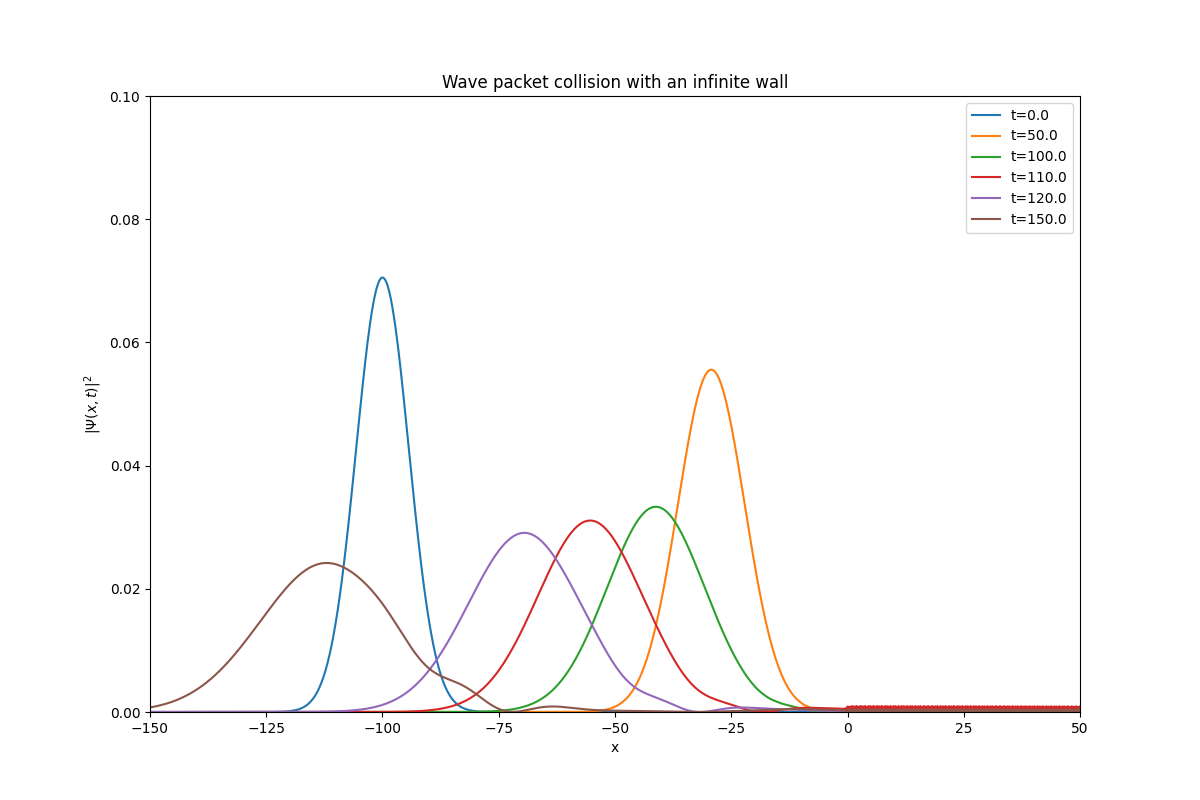
\includegraphics[width=0.8\textwidth]{q1_collision.png}
    \caption{Probability density $|\Psi(x,t)|^2$ at $t=0, 50, 100, 110, 120, 150$. The interference pattern is visible at $t=110$.}
    \label{fig:q1}
\end{figure}

The interference pattern observed during the collision is a \textbf{real physical effect}. It arises from the superposition of the incident and reflected components of the wave function. As the wave packet's tail still moves right while the head has reflected and moves left, constructive and destructive interference creates the observed fringes. This is characteristic of wave-particle duality and is not a numerical artifact.

\section{Question 2: Alpha Decay and Gamow Theory}
\subsection{Theory}
Alpha decay is modeled as the tunneling of an $\alpha$-particle through a Coulomb barrier. The barrier potential is:
\begin{equation}
V(x) = \begin{cases} -V_0 & x < R \\ C/x & x > R \end{cases}
\end{equation}
with $V_0=0, R=1, C=1$. Gamow theory predicts the transmission probability $T$:
\begin{equation}
T \approx \exp\left( -2 \int_{R}^{b} \sqrt{\frac{2m}{\hbar^2}(V(x)-E)} dx \right) \propto \exp\left( -\frac{K}{\sqrt{E}} \right)
\end{equation}
where $b$ is the classical turning point ($V(b)=E$).

\subsection{Results}
We simulated $E \in [0.1, 0.9]$. The transmission $T$ was calculated from the maximum amplitudes $Y_T$ (transmitted) and $Y_R$ (reflected) at $t_{max}$ such that the packets have fully separated.
\begin{figure}[ht]
    \centering
    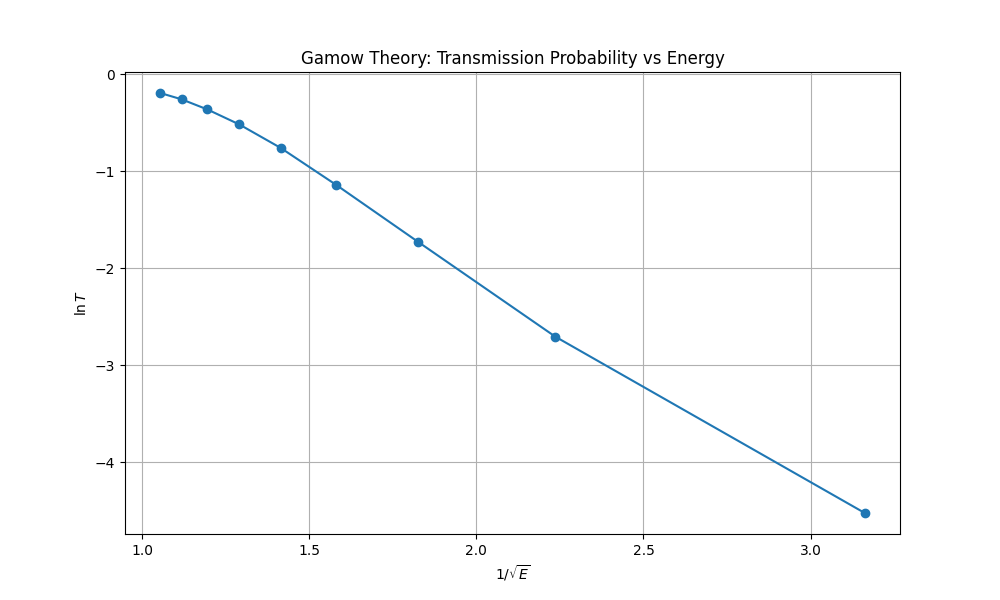
\includegraphics[width=0.6\textwidth]{q2_gamow.png}
    \caption{Verification of Gamow's law: $\ln T$ vs $1/\sqrt{E}$ shows a linear relationship.}
    \label{fig:q2}
\end{figure}
As shown in Figure \ref{fig:q2}, the plot of $\ln T$ vs $1/\sqrt{E}$ yields a straight line, confirming the exponential dependence of decay rates on energy predicted by Gamow.

\section{Question 3: Fowler-Nordheim Tunneling}
\subsection{Theory}
Field emission occurs when an external electric field $\mathcal{E}$ lowers the barrier at a metal surface, allowing electrons to tunnel out. The potential is modeled as:
\begin{equation}
V(x) = \begin{cases} 0 & x < 0 \\ V_0 - e\mathcal{E}x & 0 < x < L \\ 0 & x > L \end{cases}
\end{equation}
The WKB approximation for a triangular barrier gives:
\begin{equation}
T \propto \exp\left( -\frac{4\sqrt{2m} V_0^{3/2}}{3e\hbar\mathcal{E}} \right)
\end{equation}
implying $\ln T \propto -V_0^{3/2}$ for a fixed field.

\subsection{Results}
We first demonstrated total reflection for $E < V_0$ without a field. Applying a linear potential $V(x) = V_0(1-x/L)$ with $L=4$ enabled tunneling. 
\begin{figure}[ht]
    \centering
    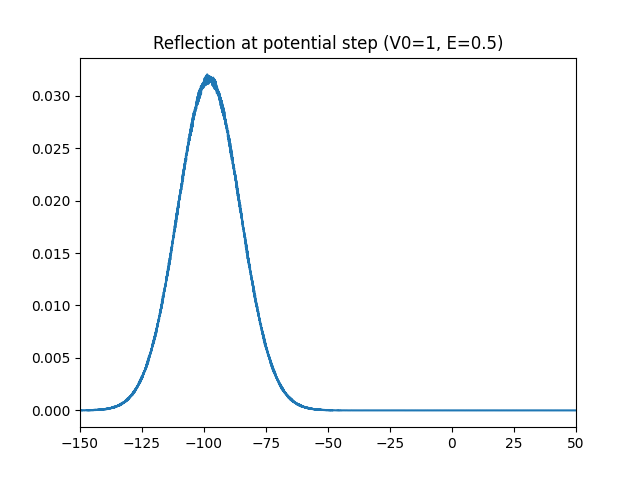
\includegraphics[width=0.45\textwidth]{q3_step_reflection.png}
    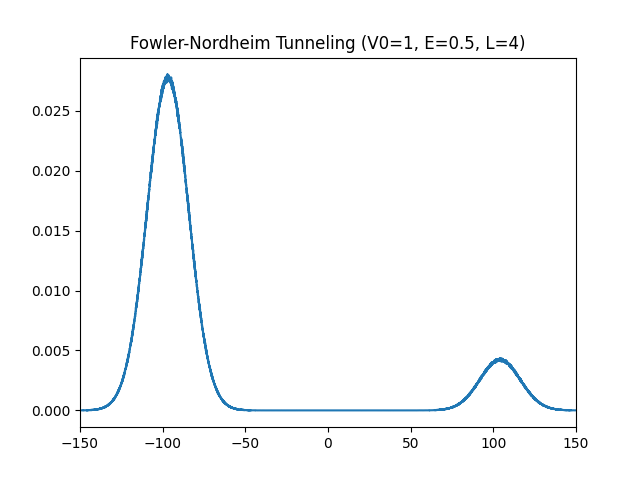
\includegraphics[width=0.45\textwidth]{q3_fn_tunneling.png}
    \caption{Left: Total reflection at a potential step ($V_0=1, E=0.5$). Right: Tunneling through the FN barrier.}
    \label{fig:q3_demo}
\end{figure}
We varied $V_0$ from $0.6$ to $1.2$ at fixed $E=0.4$. The resulting plot of $\ln T$ vs $V_0^{3/2}$ (Figure \ref{fig:q3_scaling}) is linear, confirming the Fowler-Nordheim scaling.
\begin{figure}[ht]
    \centering
    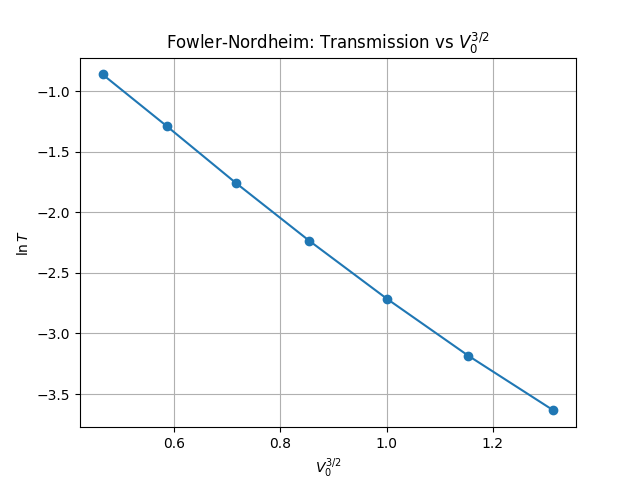
\includegraphics[width=0.6\textwidth]{q3_fn_scaling.png}
    \caption{Scaling of $\ln T$ with $V_0^{3/2}$ for field emission.}
    \label{fig:q3_scaling}
\end{figure}

\section{Conclusion}
The Split Operator Method proved to be a robust tool for simulating quantum dynamics. We successfully validated Gamow's theory of alpha decay and the Fowler-Nordheim law for field emission, demonstrating the power of numerical methods in exploring phenomena where analytical solutions are complex.

\end{document}
